% Chapter 4 - Results
%   Tool Implementation
% 	Profiling final product
% 	Measuring the Hypothesis

%- Guide (250-1000 Words)

\chapter{Results}
\label{chap:chapter4}
To better explain each result the order that was described in the methodology section will not be followed.
First the implementation of the tool will be discussed, followed by issues encountered in development and finally comparisons between results from the Aletheia platform and existing file carving programs.

\section{Tool Implementation}
\label{sec:PFACResults}
As mentioned above in the methodology, implementation was split into two sections that worked together to become the final file header/footer search.
These two sections can be seen in the GitHub Repositories, \href{https://github.com/yeroc-sebrof/fileChunkingClass}{yeroc-sebrof/fileChunkingClass} and \href{https://github.com/yeroc-sebrof/Aletheia}{yeroc-sebrof/Aletheia}.
Development of the tool was performed through milestones as a staged development process, as expected of \acl{RAD}.
This iterative process was effective in the creation of the final tool.

The results from the \ac{CPU} versions of the tool show insight as to the improvement in not only the development of the tool but that comes with the use of \ac{GPGPU} methods.
When comparing these tools to the existing Foremost and Scalpel tools that are later tested it is clear to what extent the \ac{PFAC} algorithm is ill fitted to CPU execution.
Appendix \ref{sec:PFACappendix} contains said results from each main stage of the \ac{CPU} tools development as well as links to the code repositories.

\section{Evaluation of the final product}
\subsection{Selected File Types Searches}
\label{sec:fileTypeTest}
For testing the researcher relied on easy to generate file types.
The types that were tested for include: PNG, JPG, GIF, PDF, DOC and HTML.
File systems were then generated, of size 64\ac{MB} and these files were inserted within them to be searched for.
For this testing the chunk size for the file carver was reduced to search in 16\ac{MB} chunks.
All of these file systems tested individually against specifically compiled versions of Aletheia that would only search for the particular file type of each.

Appendix \ref{sec:fileTypeTestApp} contains the complete results of these simple tests but further testing was required due to unexpected false positives and negatives.
The encountered difficulties of false positives were acceptable; it can be considered common that stings that resemble a file header/footer can be found when they are not there for that reason.
\newpage
\subsubsection*{HTML problems}
\label{sec:HTMLissue}
Aletheias false negatives, which can be seen in Appendix \ref{subsec:fileTypeHTML}, were an issue that needed further exploration.
Due to the simplicity of this file type this issue was easy to trace.
Aletheia was modified to send the contents of the buffer where this footer should have been located to the console window.
As it can be seen in Figure \ref{fig:BadHTMLCout} this section of text did not appear as expected.

\begin{figure}[!ht]
    \centering
    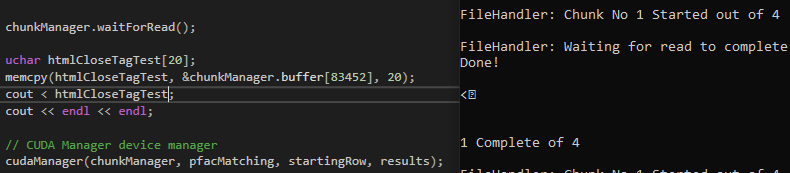
\includegraphics[width=\linewidth]{Images/Tests/64MB/MalformedClosingtag.png}
    \caption{Malformed Closing Tag}
    \label{fig:BadHTMLCout}
\end{figure}

As the pattern expected was \texttt{</html>} it was now clear why the footer was not found.
Further observation via the debug memory trace showed that the characters were not being read in correctly from the file.

\begin{figure}[!ht]
    \centering
    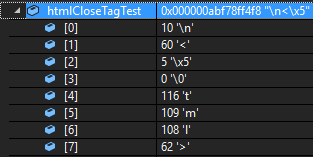
\includegraphics[width=200pt]{Images/Tests/64MB/MemoryRead.png}
    \caption{Memory Window}
    \label{fig:BadHTMLMem}
\end{figure}

Conclusions as to the source of this behaviour can be seen in the Discussion at Section \ref{subsec:fileTypeDiscussion}.

\subsection{Testing all File Types}
\label{sec:AllFileTypes}
Testing continued into searching for multiple documents through one file system of size 400\ac{MB}.
Two searches were performed but the patterns being searched for changed.
The results of this test were to determine if false positives were continuing and how many would occur in this simple example;
especially since a real world example would contain considerably more files.

The figures in Appendix \ref{sec:400MBAppendixPatterns} show the patterns that were enabled in each attempt.
This test was also able to show the speed difference obtained when less patterns were part of the search.
As you can see in Figure \ref{fig:runOnePatts}, run one was only reduced to search for patterns that could delay each thread of processing.

Overall, the tests ran without issue and the results were within expected parameters.
Said results from each run can be seen in Appendix \ref{sec:400MBAppendixResults}.

\subsection{Testing against a larger file system}
This next test was made with 10 PDFs spread out over a 2\ac{GB} disk image.
PDFs were chosen as they have been consistent to this point in returning only one header and footer.
First the disk was searched using only the PDF patterns loaded in Aletheia then the same disk image was compared to all of patterns the used in Figure \ref{fig:runOnePatts}, from the test of the 400 \ac{MB} disk.

The results that were gathered from this were very interesting and the conclusions drawn can be seen in the discussion in Section \ref{sec:400MBand2GBtookSimilarTimes}.

\subsection{Linux testing}
\label{sec:linuxResults}
All of the tests that were performed above, were then repeated on the second test environment to compare between.
The \ac{AWS} instance was used to then to provide a point of comparison to other, Linux bound, tools.

Although the \ac{SSD} was not optimal on Environment B, it was hoped that would be mitigated through the use of ram disks.
A ram disk is when a section of the main memory is assigned accessible in the same manner as backing storage drive.
Sections of testing showed that ram disks made a considerable difference to foremost but this was not a discernible difference as you can see from the results in Appendix \ref{sec:linuxTesting}, this did not have an effect on the data throughput.
Testing remained using ram disks however encase a noticeable difference could be later noticed.

Due to the shared tenancy of the \ac{AWS} instance there was an interesting set of results where the average time for the 2GB file searched for All patterns resulted in 24.512 seconds average per execution.
This test was performed again hours later for more accurate results.

\section{Comparisons to existing tools}
All of the following tests make use of the appropriate options/flags to disable the carving of the files.
These tools are only performing disk audits so the tasking is similar to Aletheias file header/footer search thus making it a fairer test.

\subsection{OpenForensics}
\label{sec:OpenForensicsComparison}
Although seldom mentioned up to this point, the only tool that was found in open-source that makes use of \ac{GPGPU} methods for file carving OpenForensics was used to compare against.
OpenForensics, authored by Dr Bayne is the testing platform mentioned in the paper ``Accelerating Digital Forensic searching through \ac{GPGPU} Parallel Processing Techniques'' (Bayne, 2017).

Testing on the 400\ac{MB} and 2\ac{GB} file showed that the tool can perform at incredibly high speed on both \ac{CPU} and \ac{GPU} (as well as amalgamations of the two).
Unfortunately, issues were experienced in trying to get the 10 \ac{GB} file over from Environment B for testing in time for the final round of testing on commercial hardware was not possible.
Moreover, this testing was very limited as to the number of runs performed due to the tool being GUI driven.

The results that were gathered can be further examined in Appendix \ref{sec:OpenForensicsAppendix} and the discussion in Section \ref{sec:OpenForensicsDiscussion}.

\subsection{Foremost \& Scalpel}
\label{sec:ForemostScalpelRes}
Although both Foremost and Scalpel have windows versions, it was very difficult to compile and believed that these tools would have to function in a Linux subsystem;
which would have caused significant performance reductions making testing unfair on Environment A.
On Environment B however, for testing to take place accurate only timing was required.

The GNU utility `time' was used to measure the speed of Scalpel and Foremost on the Linux platform to the millisecond.
This utility was unable to have the output piped to a file however so manual testing was reduced to 5 runs of each tool.
Both of these tools would have recorded their time own timings but only in Seconds, so not accurate enough for this test.
A comparison using the Aletheia platform was taken to examine the added overhead to tools due to this utility which can be seen in Appendix \ref{sec:overHeadApp}.
Aletheias results from Appendix \ref{sec:overHeadApp} were included in this comparison to ensure the test is fairer.
All of the Results from these tests can be seen in Appendix \ref{sec:SNFappendix}.\\

\subsubsection*{Foremost}
Although the patterns may be different between tools, all patterns were also used as a point of comparison.

Interestingly, in testing the tool more than once, between restarts, the tool exhibited significantly faster results after test one was performed.
This was expected to be some sort of caching within either the tool or the \ac{AWS} platform.
As a result between each test of the tool, the Ubuntu instance had to be reset to ensure accurate results.